\begin{refsection}

\chapter{Investigation of \textit{NKX2.5} mutations in lymphocytic and diseased cardiac tissue DNA}
\chaptermark{Investigation of \protect \textit{NKX2.5} mutations}
\label{Chapter5}

\section{Introduction}
Transcription factors are increasingly recognized as having key roles in the complex biological processes governing cardiac development \cite{akazawa2005cardiac,benson1999mutations}. Of the various genes implicated mutations in cardiac transcription factor \textit{NKX2.5} has been identified in both familial and sporadic CTHD cases \cite{goldmuntz2001nkx2,reamon2004somatic,reamon2004novel}.

The \textit{NKX2.5} gene is the master regulator of the process of cardiogenesis. It belongs to the \textit{NK2} family of homeobox genes and is a homolog of the tinman found in \textit{Drosophila melanogaster}. The gene maps to chromosome 5q34 and is made up of two exons with the homeodomain region being present on exon 2. Two other domains, the transactivation and NK-2-specific domains, are highly conserved and have autoregulatory functions \cite{inga2005functional}. Molecular dissection of the gene has revealed the participation of highly conserved regions in DNA binding, protein-protein interactions, nuclear translocation, and regulation of other transcription factors \cite{grow1998tinman,kasahara2004biochemical,kasahara2000loss,kasahara2001progressive}.

Till date, over 40 heterozygous mutations, both synonymous and non-synonymous have been identified in the \textit{NKX2.5} gene, resulting in various CHD phenotypes \cite{reamon2004somatic,reamon2004novel,mcelhinney2003nkx2}. A few SNP have also been reported, which appear to be specific to Asian populations and not seen frequently elsewhere \cite{dinesh2010single}. Furthermore, previous studies have revealed that \textit{NKX2.5} mutations may be mosaic in nature, meaning that they are confined to the affected tissue and, hence, not detected in a simple blood analysis \cite{reamon2004somatic,reamon2004novel}. The significance of this hypothesis is now being acknowledged, but rarely studied.

During cardiovascular development, optimal \textit{NKX2.5} gene expression is an important requisite \cite{pabst2008novel}, owing to the dosage interdependence between cardiac transcription factors, and hence, the proper development of cardiac structures. In a recent study by Sheng et al \cite{sheng2013dna}, mRNA levels of the \textit{NKX2.5} were significantly lower in TOF patients compared to controls.

Owing to the functional significance and emerging insights, mutations in the \textit{NKX2.5} gene in the selected study population was studied in DNA obtained from both blood and the cardiac tissue of cases with CTHD. The variations seen in the genotypes and gene expression between blood and cardiac tissue samples for each of these individuals were also examined. In order to corroborate that any of the sequence alterations observed were mutations, lymphocytic DNA from controls was used.

\section{Methodology}


\begin{table}[!tb]
\centering
\caption{PCR primers and reaction conditions used to amplify \textit{NKX2.5} \cite{goldmuntz2001nkx2}}
\label{tab:5_1}
\begin{tabular}{  P{0.5in} P{1in} P{0.5in} l }
\toprule
	\textbf{Exon} & \textbf{Amplicon size (bp)} & \textbf{Tm (ºC)}  & \textbf{Primer sequence} \\ \toprule
	1A & 404 & 62º & F:5’ CGG CAC CAT GCA GGG AAG 3’ \\ 
	 &  &  & R:5’ AGG GTC CTT GGC TGG GTC GG 3’ \\ \midrule
	1B & 355 & 67.5 & F:5’ CCT AAA CCT GGA ACA GCA GC 3’ \\ 
	 &  &  & R: 5’ TCC TGG CCC TGA GTT TCT TG  3’ \\ \midrule
	2A & 469 & 67.5 & F:5’ TAG GGA TTG AGG CCC ACG 3’ \\ 
	 &  &  & R: 5’TAG GGA TTG AGG CCC ACG 3’ \\ \midrule
	2B & 442 & 67.5 & F:5’ CAG ACT CTG GAG CTG GTG G \\ 
	 &  &  & R:5’ CCC ACG AGA GTC AGG GAG 3 ‘ \\ \bottomrule
\end{tabular}
\end{table}

DNA was isolated from the blood of the 96 cases and 100 controls as detailed in Section 2.3.3. Additionally, DNA was isolated from the tissue obtained as surgical discards from 55 patients as described in Section 2.3.4. The coding region, including exon/intron boundaries, was amplified from genomic DNA with sequence specific primers as two overlapping sequences for each exon (\cref{tab:5_1}). All reactions started with 2 minutes at 95°C followed by 35 cycles of 45 seconds at 95°C, 30 seconds at 60°C (exon 1A) or 67.5 °C (exon 1B,2A,2B), and 45 seconds at 72°C and finished with a 10-minute extension period at 72°C. DMSO (0.5 mL/20µL reaction) was added for the reactions. The amplicons were purified using exosap and then were fractionated on an ABI3730 automated DNA sequencer and analyzed using the SeqScape analysis software V2.5.

Total RNA was isolated from the peripheral blood and cardiac tissue samples using the TRIzol method as outlined in section 2.3.5.The isolated RNA was converted to cDNA and subjected to real-time PCR using SYBR Green chemistry (Applied Biosystems) with specific primers (\cref{tab:5_2}) under the standard conditions of 95ºC for 10min, 60 ºC for 20s, and data collection at 72 ºC in Applied Biosystems 9700 HT. β-actin was used as an endogenous control, and the amount of target gene normalized to β -actin was determined by the delta C$_t$ method.


\begin{table}[!tb]
\centering
\caption{Primer sequence used for RT PCR \cite{sheng2013dna}}
\label{tab:5_2}
\begin{tabular}{  P{1in} P{1in} l }
\toprule
	\textbf{Gene} & \textbf{Product length (bp)} & \textbf{Primer} \\ \toprule
	\textit{NKX2.5} & 21 & F: 5’ GGG CCT CAA TCC CTA CGG TTA 3’ \\ 
	 &  & R: 5’ CCG AAG TTC ACG AAG TTG TTG 3’ \\ \bottomrule
\end{tabular}
\end{table}

\section{Results}

\subsection{\textit{NKX2.5} mutations in blood}

\begin{sidewaysfigure}[!hp]
\centering
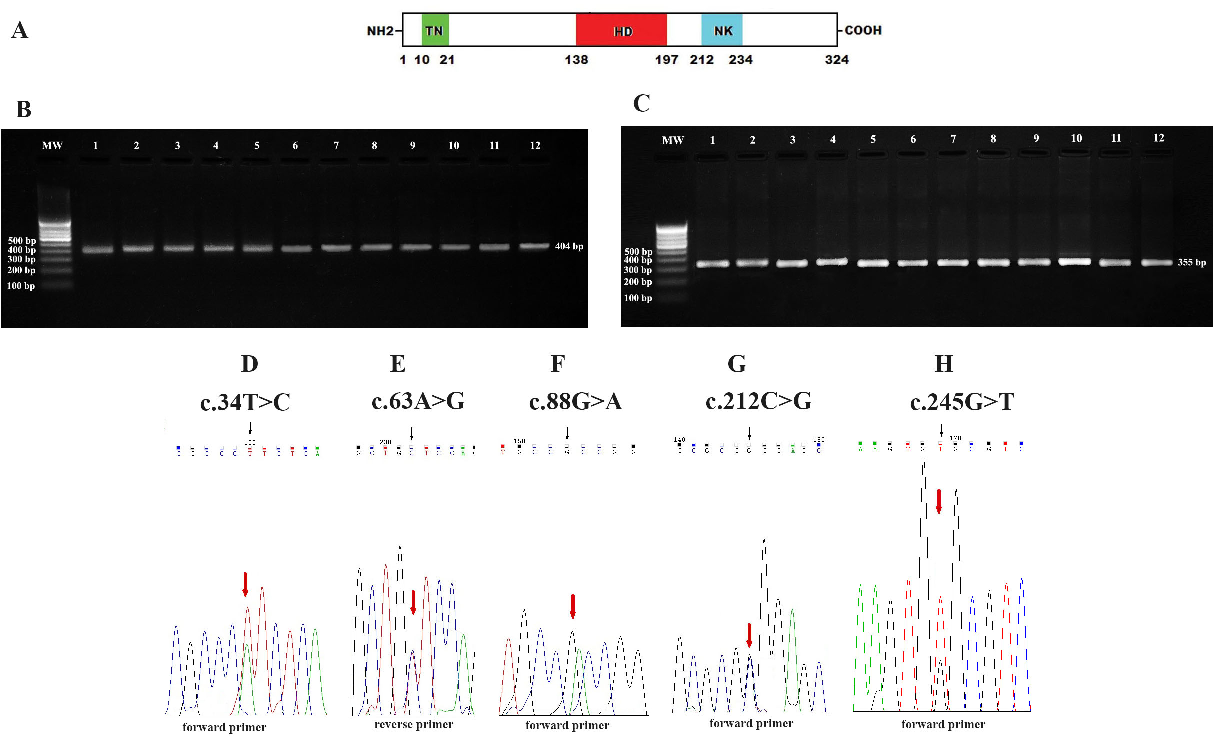
\includegraphics[scale=0.95,keepaspectratio]{Figures/Figure5_1.pdf}
\rule{35em}{0.5pt}
\caption{\textbf{\textit{NKX2.5} mutations observed in exon 2}. \textbf{A.} Schematic representation of the \textit{NKX2.5} gene. \textbf{B,C.} 2\% agorse gel images showing the representative amplicons of \textit{NKX2.5} exon 1A (404bp) and exon1B (355bp) respectively \textbf{D-I.} Sequence chromatograms of \textit{NKX2.5} sequence variants detected in exon 2 of index cases. Arrows indicate the heterozygous nucleotides of c.34T>C, c.63A>G, c.88G>A, c.212C>G and c.245G>T}
\label{fig:5_1}
\end{sidewaysfigure}

\begin{sidewaysfigure}[!hp]
\centering
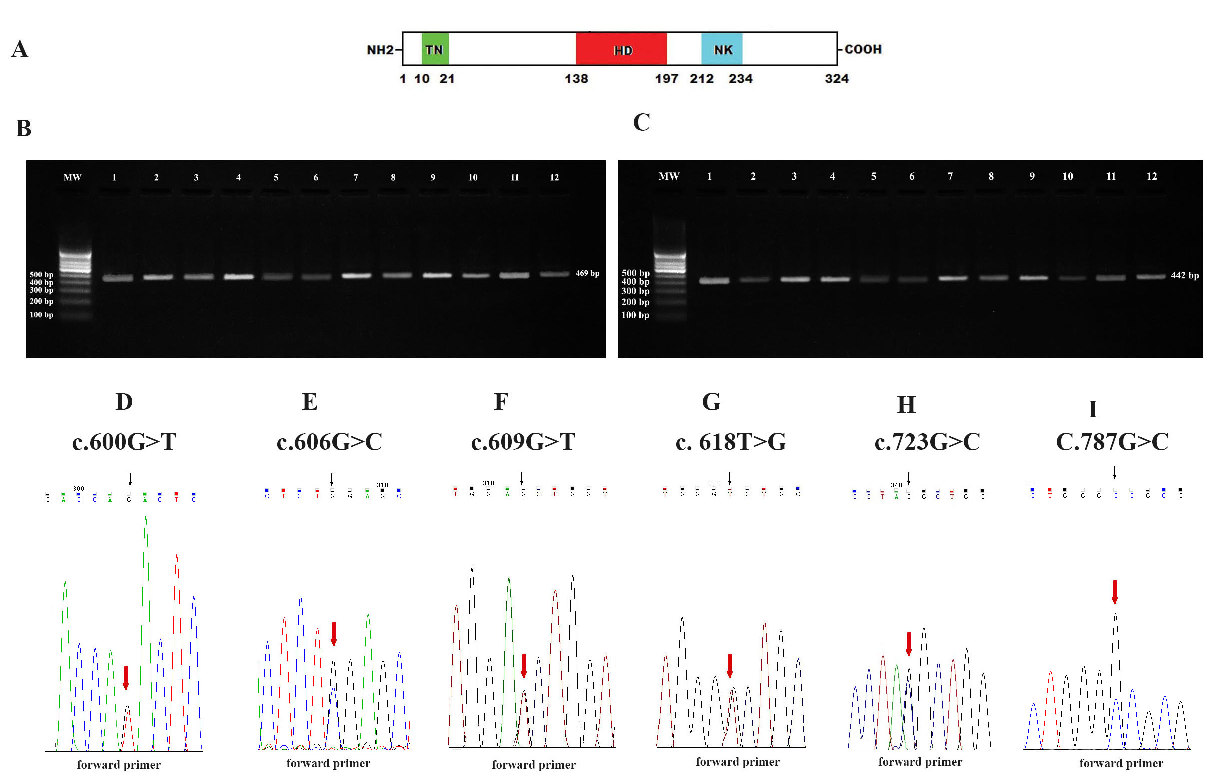
\includegraphics[scale=0.9,keepaspectratio]{Figures/Figure5_2.pdf}
\rule{35em}{0.5pt}
\caption{\textbf{\textit{NKX2.5} mutations observed in exon 2.} \textbf{A.} Schematic representation of the \textit{NKX2.5} gene. \textbf{B,C.} 2\% agorse gel images showing the representative amplicons of \textit{NKX2.5} exon 2A (469bp) and exon2B (442bp) respectively \textbf{D-I.} Sequence chromatograms of \textit{NKX2.5} sequence variants detected in exon 2 of index cases. Arrows indicate the heterozygous nucleotides of c.600G>T, c.606G>C, c.609G>T, c.618T>G, c.723C>G and c.787G>C}
\label{fig:5_2}
\end{sidewaysfigure}

Eleven heterozygous sequence variants, predicted to alter the encoded protein, were identified in the lymphocytic DNA of 21 unrelated cases of CTHD (\cref{fig:5_1,fig:5_2}). Eight of the 11 sequence variants observed had single nucleotide changes that would result in an amino acid change (non-synonymous mutations). None of these mutations were observed in the controls. The total prevalence of \textit{NKX2.5} mutations in the study population was approximately 10.4\%. 
The disease-causing potential of the observed sequence alterations was predicted using the MutationTaster program (15), which would suggest whether alteration could either be a disease mutation or a harmless polymorphism. The sequence alterations of c.723C>G, c.34T>C, c.600G>T and c.609G>T were all predicted to be disease-causing. The remaining sequence alterations were predicted to be benign polymorphisms. The results of the bidirectional sequencing are summarized in \cref{tab:5_3}.



All the cases that were mutation positive (\cref{tab:clinchar}) did not have a significant family history and were born of non-consanguineous marriages (NCM). Seven of the 21 cases had extracardiac features in addition to a CTHD.

\subsection{\textit{NKX2.5} mutations in tissue}

About 11\% of the cases showed a heterozygous single nucleotide change of C to A at codon position 195 and included cases \#2, 3, 34, 37, 40, 47 (\cref{fig:5_3}). Additionally, two frameshift mutations caused by a deletion of nucleotide A at codon position 139 and 155 were observed in a case of TOF (\cref{fig:5_4}). Neither the synonymous mutation nor the deletions were observed in the lymphocytic DNA of the cases or among the controls.

\begin{figure}[!htb]
\centering
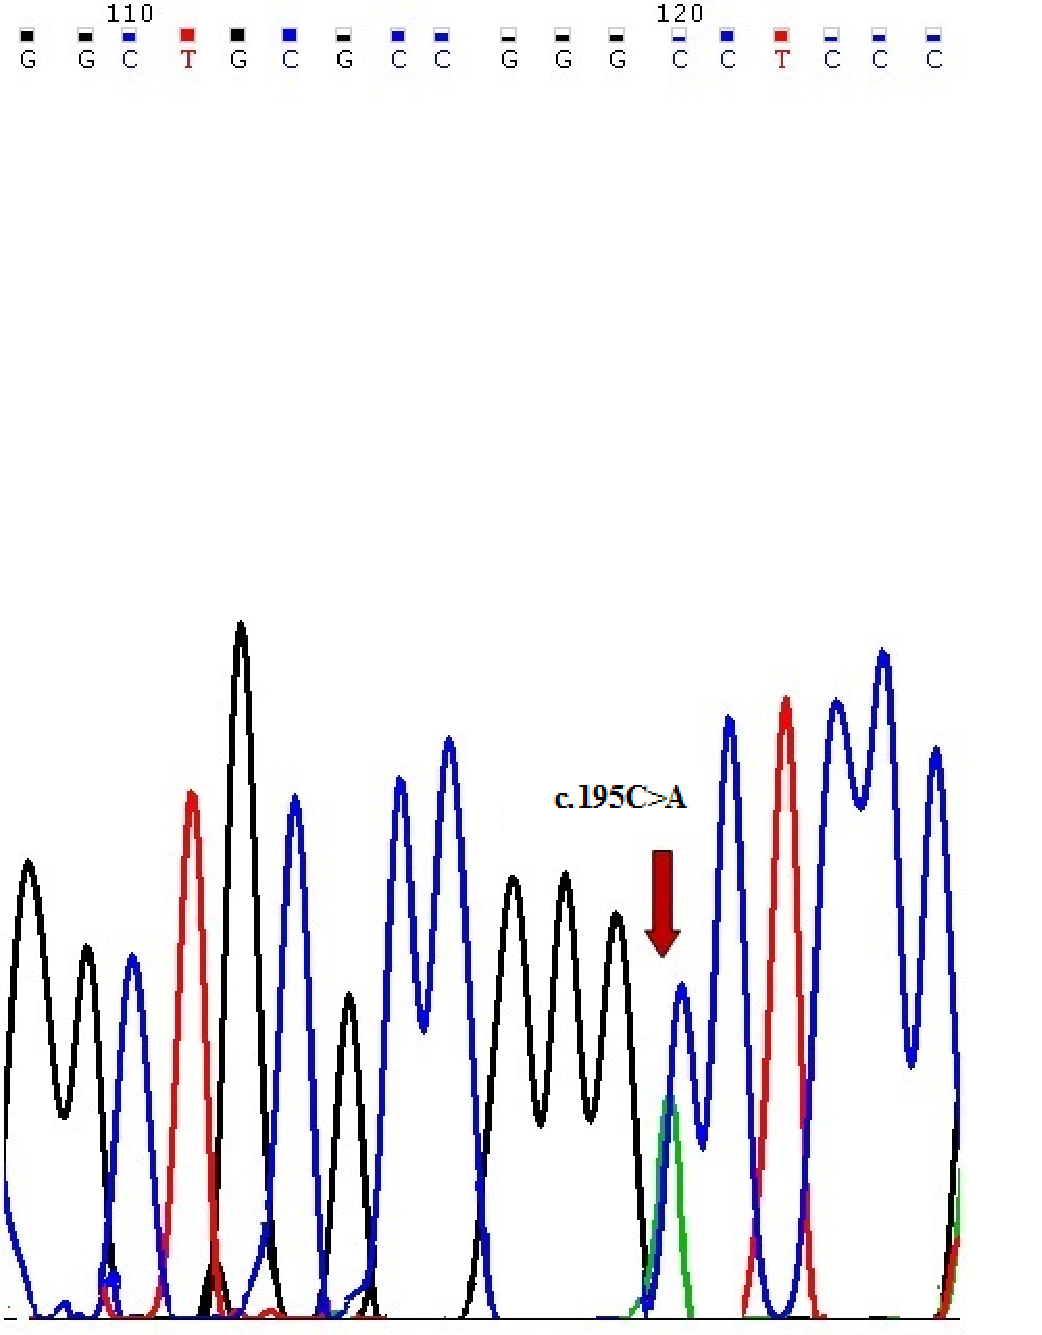
\includegraphics[scale=0.5,keepaspectratio]{Figures/Figure5_3.pdf}
\rule{35em}{0.5pt}
\caption{Sequence chromatogram showing the \textit{NKX2.5} heterozygous sequence variant \textbf{c.195C>A} identified in the cardiac tissue of six cases}
\label{fig:5_3}
\end{figure}



\begin{landscape}
\begin{table}[!p]
\renewcommand{\arraystretch}{1.2}
\centering
\caption{Summary of \textit{NKX2.5} mutations detected in blood}
\label{tab:5_3}

\begin{tabular}{ P{0.75in} P{0.85in} P{0.75in} P{2.25in}  p{3.85in} }
\toprule
	\textbf{Nucleotide change} & \textbf{GenBank Accession} \# & \textbf{AA change} & \textbf{No. of genotype positive patients} & \textbf{Prediction} \\ \toprule
	c.34T>C & - & Phe>Leu & 3: Case \#28, 30,38 & Disease causing; amino acid sequence changed \\ \midrule
	c.63A>G & - & Gln>Glu  & 8 : Case \#3,4,6,14,26,28,36,38 & Polymorphism; protein features (might be) affected ,splice site changes \\ \midrule
	c.88G>A & KT984167 & Ala>Pro & 2: Case \#36,48 & Polymorphism; protein features (might be) affected ,splice site changes \\ \midrule
	c.212C>G & KT984165 & Ala>Gly & 1: Case \#66 & Polymorphism; amino acid sequence changed, protein features (might be) affected \\ \midrule
	c.245G>T & KT984166 & Cys>Phe & 2: Case \#66,84 & Polymorphism; amino acid sequence changed, protein features (might be) affected \\ \midrule
	c.600G>T & KT984164 & Gln>His & 10: Case \#52,54,56,57,58,67,68,69,70,71 & Disease causing; amino acid sequence changed \\ \midrule
	c.606G>C & KT984164 & Leu>Leu & 1: Case \#69 & Polymorphism; homozygous in TGP \\ \midrule
	c.609G>T & KT984164 & Glu>Asp & 1: Case \#69 & Disease causing; amino acid sequence changed \\ \midrule
	c.618T>G & - & Gly>Gly & 1: Case \#69 & Polymorphism; homozygous in TGP:  \\ \midrule
	c.723C>G & - & Tyr>X & 1: Case \#66 & Disease causing; amino acid sequence changed, splice site changes ,truncated protein (might cause NMD) \\ \midrule
	c.787G>C & - & Gly>Gly & 2: Case \#66,84 & Polymorphism; amino acid sequence changed, protein features (might be) affected \\ \bottomrule
	\multicolumn{5}{l}{\textsuperscript{*}\footnotesize{AA: amino acid; NMD :  nonsense-mediated mRNA decay;TGP: 1000 Genomes Project}}\\
\end{tabular}
\end{table}
\end{landscape}

\begin{landscape}
\begin{spacing}{1}

\begin{longtable}{p{0.5in} p{0.5in} p{1in} p{3in} p{3in}}

%\centering
\caption{Clinical characteristics of mutation positive cases}\\

%\begin{tabular}
           \toprule
          \textbf{S. No}
        & \textbf{Case}
        & \textbf{Age/Gender}
        & \textbf{Cardiac Findings}
        & \textbf{Extra-cardiac finding}
        \\* \toprule
	\endhead
 \label{tab:clinchar}  
   	
	1.  & \# 3 & 1y3m/M & TGA with situs solitus, levocardia and predominant infundibular stenosis & Not present \\ \midrule
	2.  & \# 4 & 1y10m/M & TGA with situs solitus, levocardia and predominant infundibular stenosis & long narrow face, hooded eyelids, rectangular nose, small mouth, delayed development, failure to thrive \\ \midrule
	3.  & \# 6 & 8y/M & TGA and aortic failure  & Not present \\ \midrule
	4.  & \# 14 & NB/M & TA with right aortic arch, stenosis truncal valve and PA stenosis & Not present \\ \midrule
	5.  & \# 26 & 11y/F & TOF & Not present \\ \midrule
	6.  & \# 28 & 3y6m/F & TA with right aortic arch,stenosis truncal valve and PA stenosis & Not present \\ \midrule
	7.  & \# 30 & 1y6m/F & TOF with stenosis of the right branch of the pulmonary artery & Not present \\ \midrule
	8.  & \# 36 & 1y7m/F & IAA with hypoplastic infantibular septum and subarterial VSD & Not present \\ \midrule
	9.  & \# 38 & 7y3m/F & TOF with stenosis of the right branch of the pulmonary artery & Not present \\ \midrule
	10.  & \# 48 & 1y7m/M & IAA with hypoplastic pulmonary valve and hypoplastic infundibulum & long narrow face, hooded eyelids \\ \midrule
	11.  & \# 52 & 15y8m/M & TOF with pulmonary collaterals and a large subaortic VSD & gross milestones delay \\ \midrule
	12.  & \# 54 & 18y/M & TOF with left aortic arch and a large subaortic VS & long narrow face, rectangular nose, small abnormal ears, long slender fingers, prognatinism, high arch palate, ENT anomaly, failure to thrive \\ \midrule
	13.  & \# 56 & 1y2m/F & TOF with interventricular communication & Not present \\ \midrule
	14.  & \# 57 & 1y9m/M & TA with right aortic arch, stenosis truncal valve and PA stenosis & Not present \\ \midrule
	15.  & \# 58 & 2y/F & TOF with large malaligned subaortic VSD and severe infundibular stenosis & flat malar bones \\ \midrule
	16.  & \# 66 & 3y6m/M & TOF & Not present \\ \midrule
	17.  & \# 67 & 2y/M & TOF with right aortic arch and large malaligned subaortic VSD   & long narrow face, flat malar bones, small chin \\ \midrule
	18.  & \# 68 & 1y6m/M & DORV with left aortic arch, mid doming valve, severe infundibular septum and supravalvar narrowing & Not present \\ \midrule
	19.  & \# 69 & 2m/F & TA with right aortic arch, stenosis truncal valve and PA stenosis & Not present \\ \midrule
	20.  & \# 70 & 18y/M & DORV with left aortic arch, hypoplastic annulus, hypoplastic infundibulum and large subarterial VSD  & long narrow face \\ \midrule
	21.  & \# 71 & 15y & TOF & Not present \\ \bottomrule
%\end{tabular}
\end{longtable}
\end{spacing}
\end{landscape}

\begin{figure}[!htb]
\centering
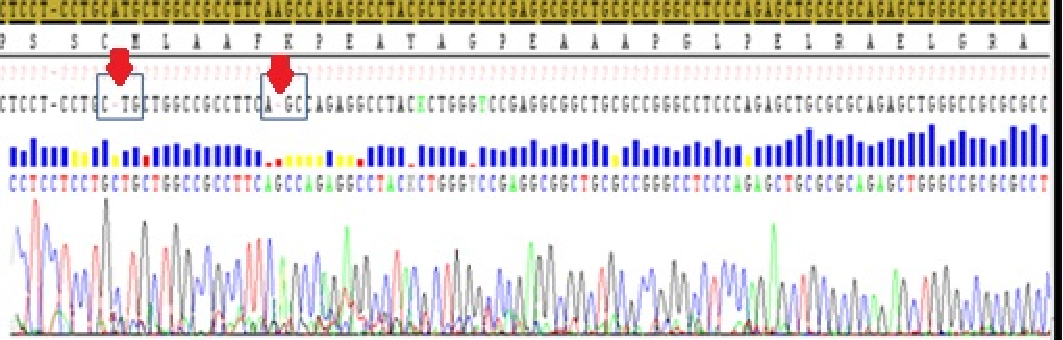
\includegraphics[scale=0.75,keepaspectratio]{Figures/Figure5_4.pdf}
\rule{35em}{0.5pt}
\caption{Sequence chromatogram showing two deletion mutations identified in a case of TOF, \textbf{c.139\_139delA} and \textbf{c.155\_155delA} as indicated by the arrow}
\label{fig:5_4}
\end{figure}

Five of the 7 cases that were mutation positive (\cref{tab:5_5}) did not have a significant family history and were born of non-consanguineous marriages (\cref{tab:5_6}). Case \# 31 was the first live born of a NCM with the mother having two spontaneous abortions before the birth of the proband. Also, the father presented with small palberal fissures and flattened nasal bone. Case \#34 was the third child of a consanguineous marriage. However the siblings did not have any history of CHD.


\begin{table}[!tb]
\centering
\caption{Summary of \textit{NKX2.5} mutations detected in diseased cardiac tissue}
\label{tab:5_5}
\begin{tabular}{  p{1.25in} p{0.75in} p{3in} }
\toprule
	\textbf{Nucleotide change} & \textbf{AA change} & \textbf{Prediction} \\ \toprule
	c.195C>A & Gly>Gly & Disease causing; protein features (might be), affected, splice site changes \\ \midrule
	c.139\_139delA & Met>Cys fs*129 & \multirow{2}{3in}{Disease causing; amino acid sequence changed, frameshift, protein features might be affected splice site changes, truncated protein might cause NMD (-150AA/more than 10\% missing)} \\ 
	c.155\_155delA & Lys>Ser  fs*124 &  \\ \bottomrule
\multicolumn{3}{l}{\textsuperscript{*}\footnotesize{fs: frameshift or further changes downstream}}\\
\end{tabular}
\end{table}

\begin{landscape}
\begin{table}[!tb]
\centering
\caption{Clinical characteristics of mutation positive cases}
\label{tab:5_6}
\begin{tabular}{ p{0.75in} p{1in} p{3in} p{3in} }
\toprule
	\textbf{Case} & \textbf{Age/ Gender}  & \textbf{Cardiac Findings} & \textbf{Extra-cardiac finding} \\ \toprule
	\# 2 & 3y2m/F & TOF with short segment narrowing, left aortic arch, hypoplastic thickened and doming, hypoplastic infundibulum, near subarterial VSD & long narrow face, flat malar bones, small chin \\ \midrule
	\# 3 & 1y3m/M & TGA with situs solitus, levocardia and predominant infundibular stenosis & Not present \\ \midrule
	\# 31 & 14y/M & TOF-age at diagnosis 8 m,TOF, absent PV, subarterial VSD,right aortic arch,left brachiocephalic vein & long narrow face,flat malar bones, small chin, narrow palpebral fissure, rectangular nose , small mouth, abnormal ears \\ \midrule
	\# 34 & 15y/M & TOF-age at diagnosis 2 years, TOF with severe infantibular ,valvar and supravalvar stenosis, right aortic arch & small chin, narrow palpebral fissure, long slender fingers \\ \midrule
	\# 37 & 18y/F & TOF- age at diagnosis 5yrs, confluent PA, right aortic arch, TOF with pulmonary atresia, retroaortic left brachiocephalic vein, supplying left lung , small collaterals & Not present \\ \midrule
	\# 40 & 1y9m/F & TGA-Situs Solitus, levocardia, AV/VA concordance, predominant infundibular stenosis & short philtrum \\ \midrule
	\# 47 & 1y6m/F & IAA- left aortic arch, severe infundibular stenosis & Not present \\ \bottomrule
\end{tabular}
\end{table}
\end{landscape}



\subsection{SNP observed in cases and controls}

The presence of a heterozygous single nucleotide change from A to G was observed in 30 cases and 7 control samples. This variation was observed at nucleotide position 63 and all three genotypes (AA, AG, GG) were seen (\cref{fig:5_5}). Codon analysis revealed that this conversion led to a synonymous substitution in codon 21, which codes for glutamic acid. This variation has already been reported in literature as the SNP rs2277923. 

According to dbSNP, the average heterozygosity of rs2277923 is 0.5 ± 0.011. Heterozygosity of the CTHD population under study is 0.242 (19 of 50 patients). 20 individuals presented with the wild type AA genotype and 11 individuals with the variant GG genotype, yielding frequencies of 0.174 and 0.084, respectively. From these frequencies (\cref{tab:5_7}), it was observed that the CTHD population followed Hardy-Weinberg equilibrium. The frequency of the SNP rs2277923 was significantly higher in the CHD population than in the control group (\cref{tab:5_8}) and distribution of the genotypes in the study population was similar to the Asian and African counterparts (\cref{fig:5_9}). 

\begin{table}[!tb]
\centering
\caption{Genotype distribution for rs2277923 in cases and controls}
\label{tab:5_7}
\begin{tabular}{  P{0.75in} P{0.75in} P{0.5in} P{0.5in} P{0.5in} P{0.5in} P{0.5in} }
\toprule
	 \multicolumn{2}{c}{\multirow{2}{2in}{}}& \multicolumn{3}{c}{\textbf{Genotype Frequency}} & \multicolumn{2}{c}{\textbf{Allele Frequency}}  \\ 
	\multicolumn{2}{c}{}   & AA & AG & GG & A & G \\ \toprule
	\multirow{2}{0.75in}{Controls (n=100)} & Observed & 86 & 14 & 0 & \multirow{2}{0.5in}{0.93}  & \multirow{2}{0.5in}{0.07} \\ 
	 & Expected & 86.5 & 13 & 0.5 &  &  \\ \midrule
	\multirow{2}{0.75in}{Cases (n=96)} & Observed & 38 & 37 & 21 & \multirow{2}{0.5in}{0.59} &  \multirow{2}{0.5in}{0.41} \\ 
	 & Expected & 33.3 & 46.5 & 16.3 &  & \\ \bottomrule
\end{tabular}
\end{table}

\begin{table}[!tb]
\centering
\caption{Analysis of rs2277923 in cases and controls}
\label{tab:5_8}
\begin{tabular}{ P{0.65in} P{0.65in} P{0.65in} P{0.65in} P{1.25in} P{0.5in}  }
\toprule
	\textbf{Genotype} & \textbf{Controls (n=100)} & \textbf{Cases (n=96)} & \textbf{Odds Ratio (OR)} & \textbf{Confidence Interval (CI)} & \textbf{p value} \\ \toprule
	AA & 86 & 38 & 1 &  &  \\ \midrule
	AG & 14 & 37 & 5.83 & 2.1126 – 16.1202 & 0.0007 \\ \midrule
	GG &  0 & 21 & 48.8 & 2.7403 – 869.20  & 0.0081 \\ \bottomrule
\end{tabular}
\end{table}

Three other SNP, namely, rs28936670, rs104893904 and rs72554029 were also studied (\cref{tab:5_9}). However, only one genotype was observed for each SNP (\cref{fig:5_6,fig:5_7,fig:5_8}) so the level of significance could not be established. But comparisons with other populations revealed a similar distribution of genotypes (\cref{fig:5_10,fig:5_11,fig:5_12}) 


\begin{figure}[!hp]
\centering
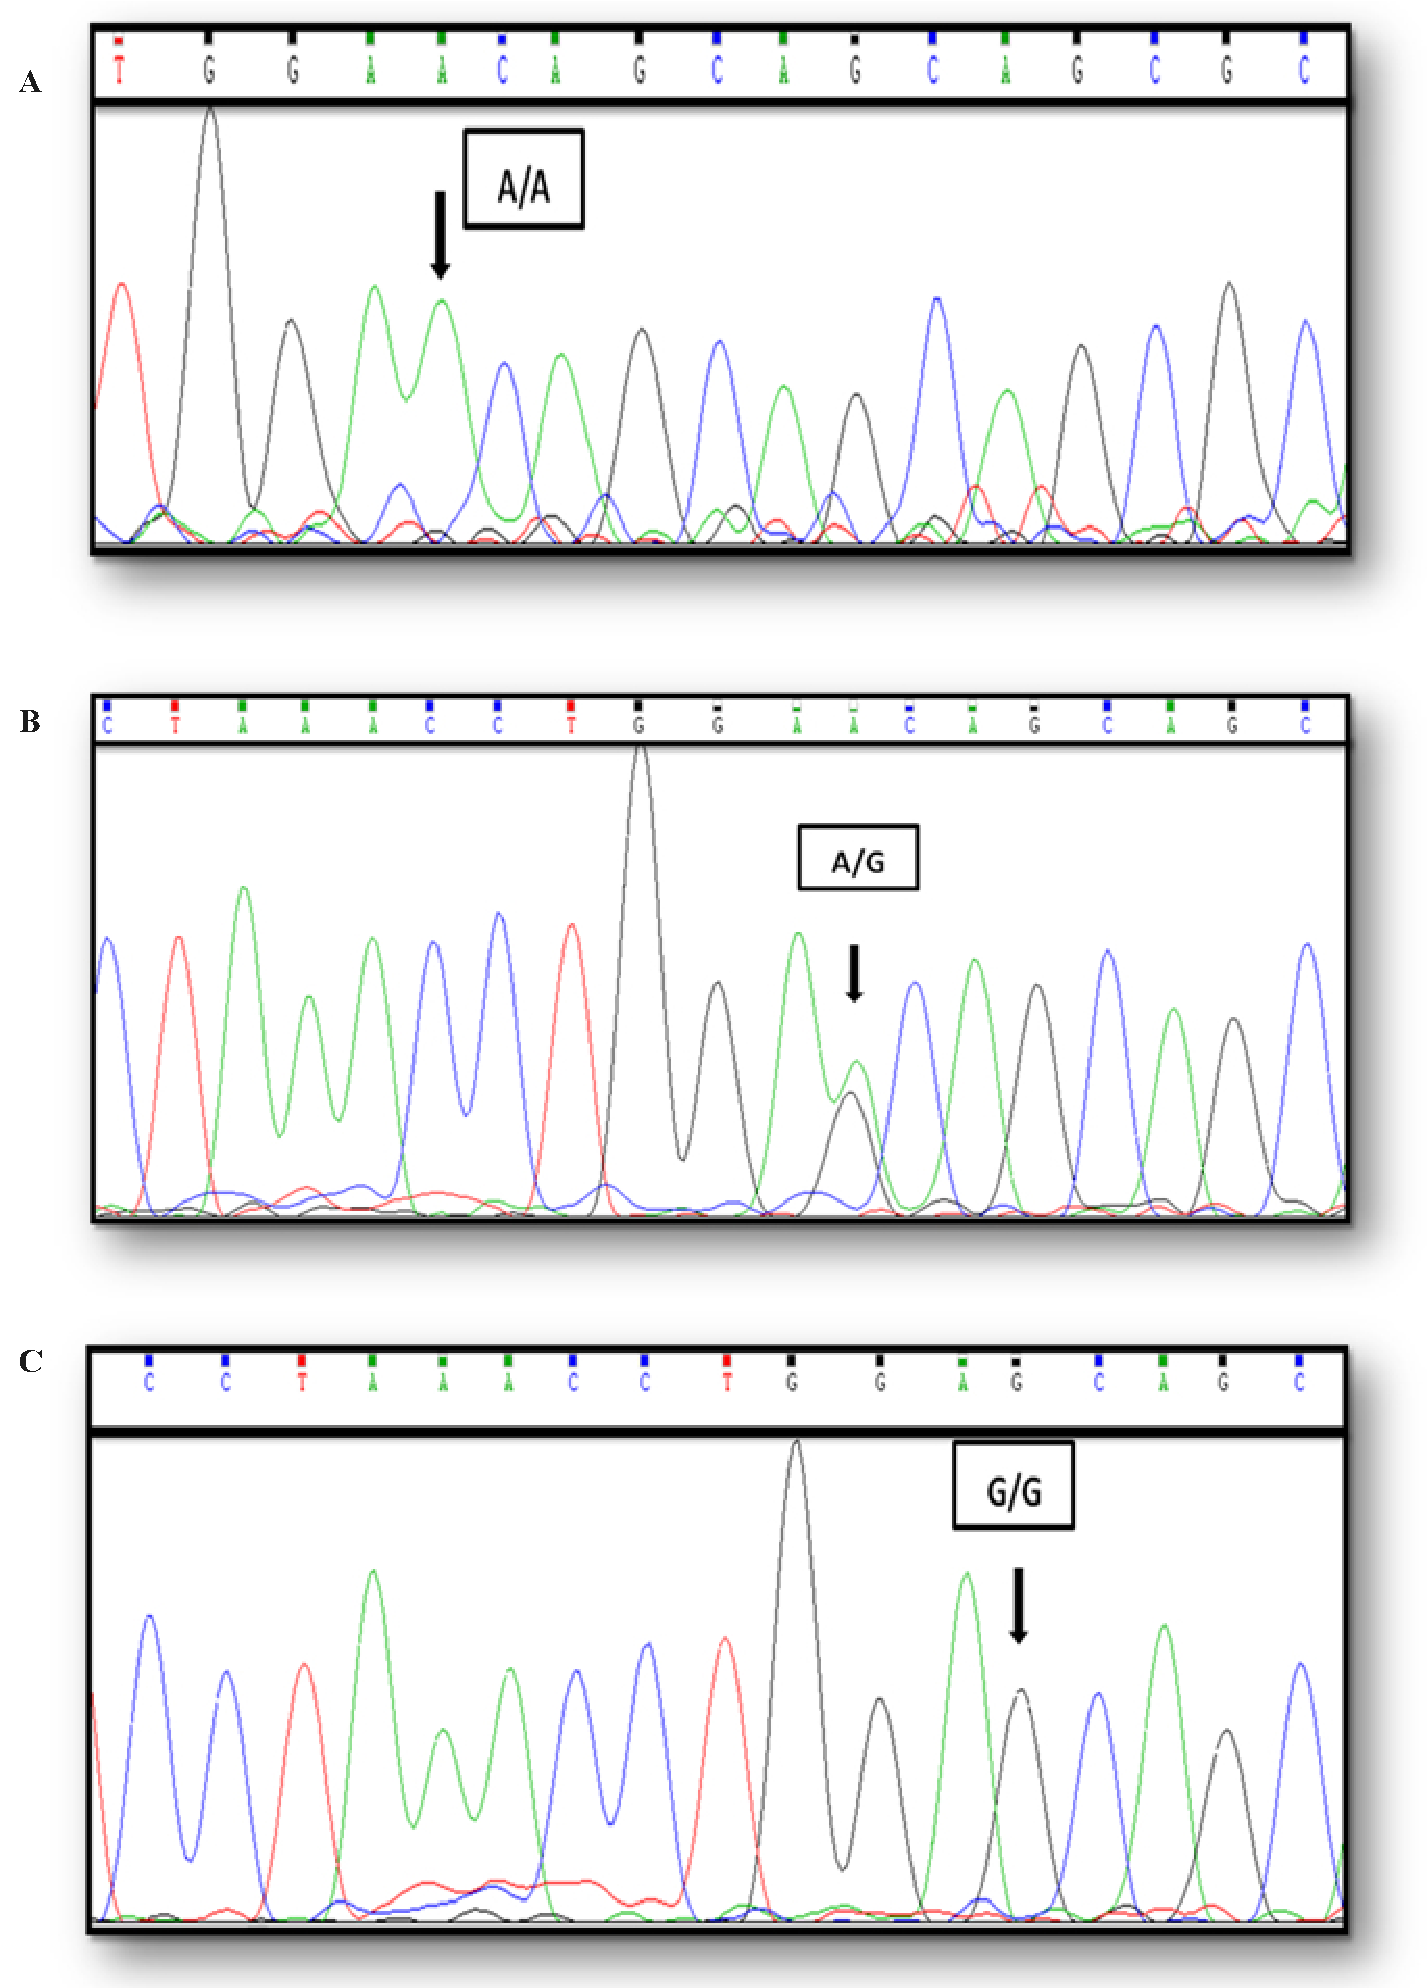
\includegraphics[width=\linewidth]{Figures/Figure5_5.pdf}
\rule{35em}{0.5pt}
\caption{Sequence chromatogram showing showing the genotypes seen for rs2277923}
\label{fig:5_5}
\end{figure}

\begin{figure}[!htb]
\centering
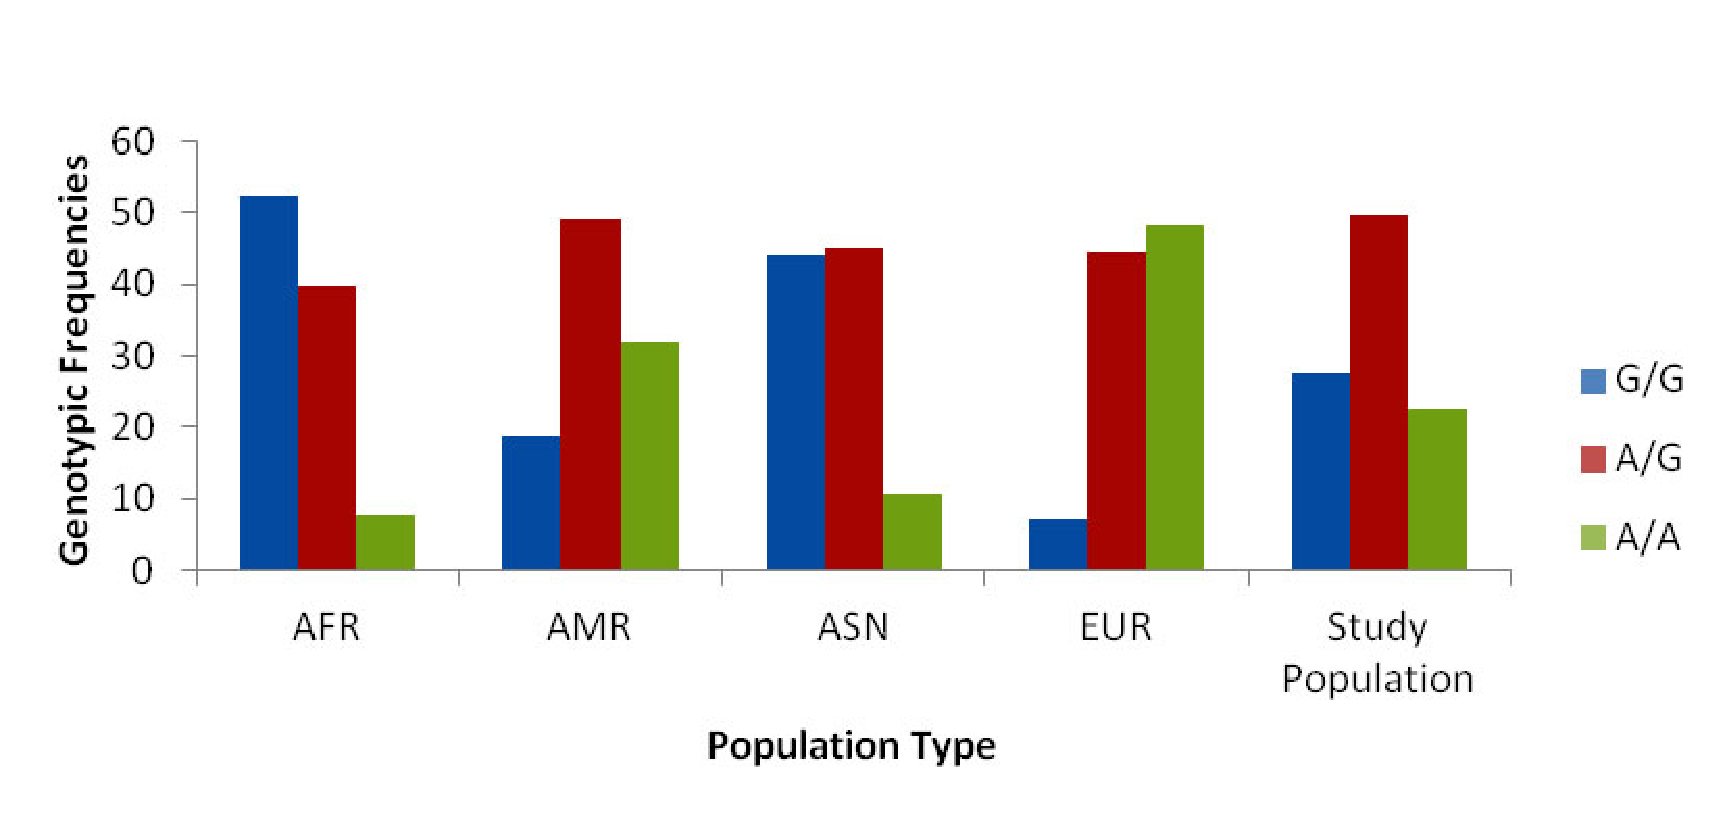
\includegraphics[width=\linewidth]{Figures/Figure5_9.pdf}
\rule{35em}{0.5pt}
\caption{Comparison of rs2277923 distribution in different populations.*\\{\textsuperscript{*}\footnotesize{AFR:African population; AMR: American; ASN: Asian and EUR: European populations}}}
\label{fig:5_9}
\end{figure}

\begin{figure}[!htb]
\centering
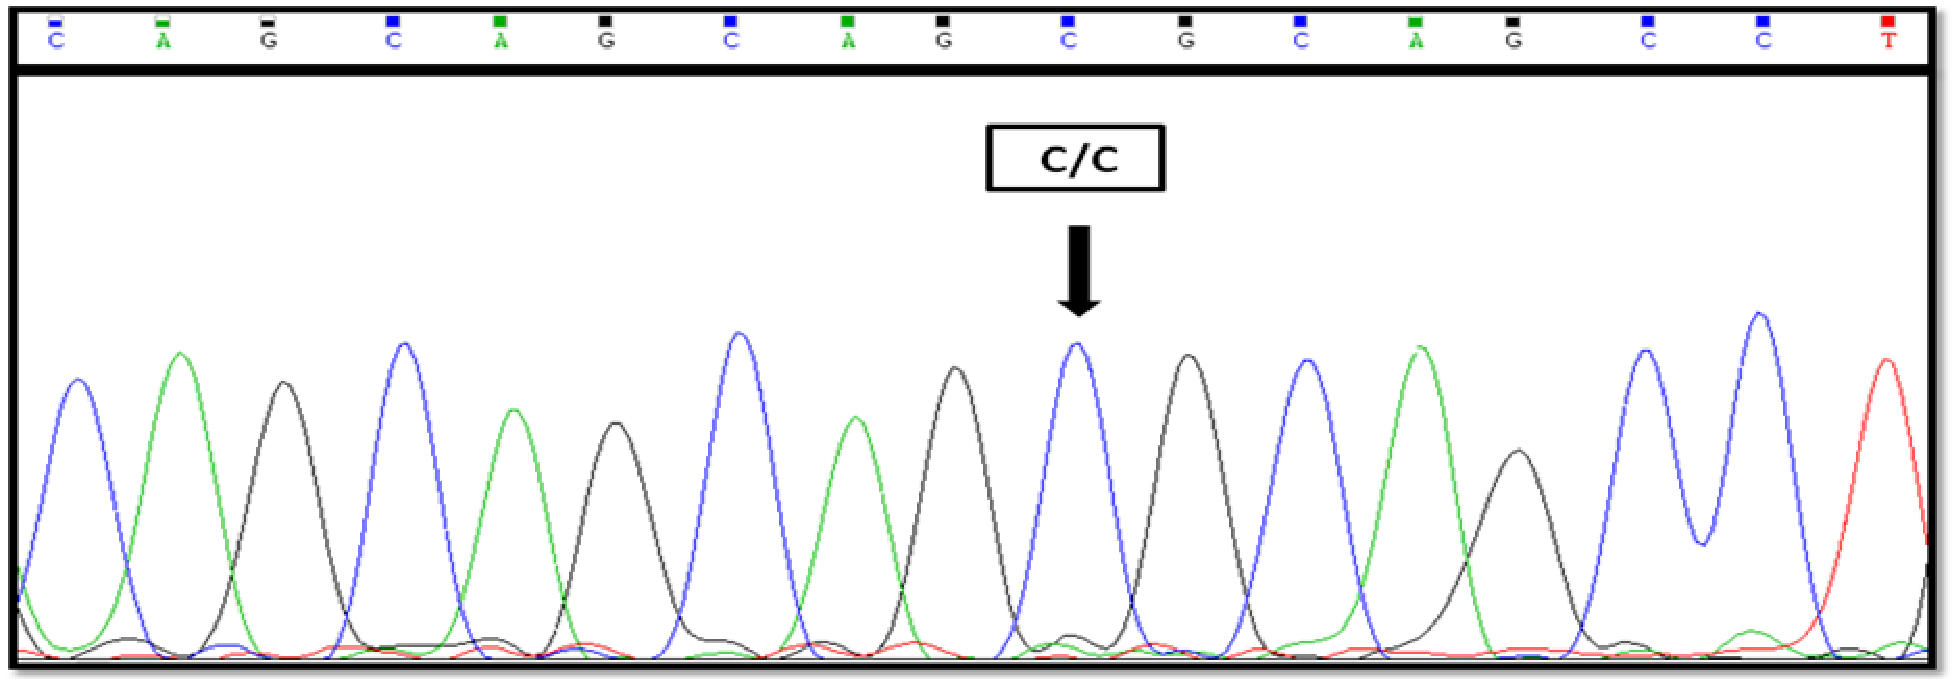
\includegraphics[width=\linewidth]{Figures/Figure5_6.pdf}
\rule{35em}{0.5pt}
\caption{Sequence chromatogram showing showing the genotypes seen for rs2277923}
\label{fig:5_6}
\end{figure}

\begin{figure}[!htb]
\centering
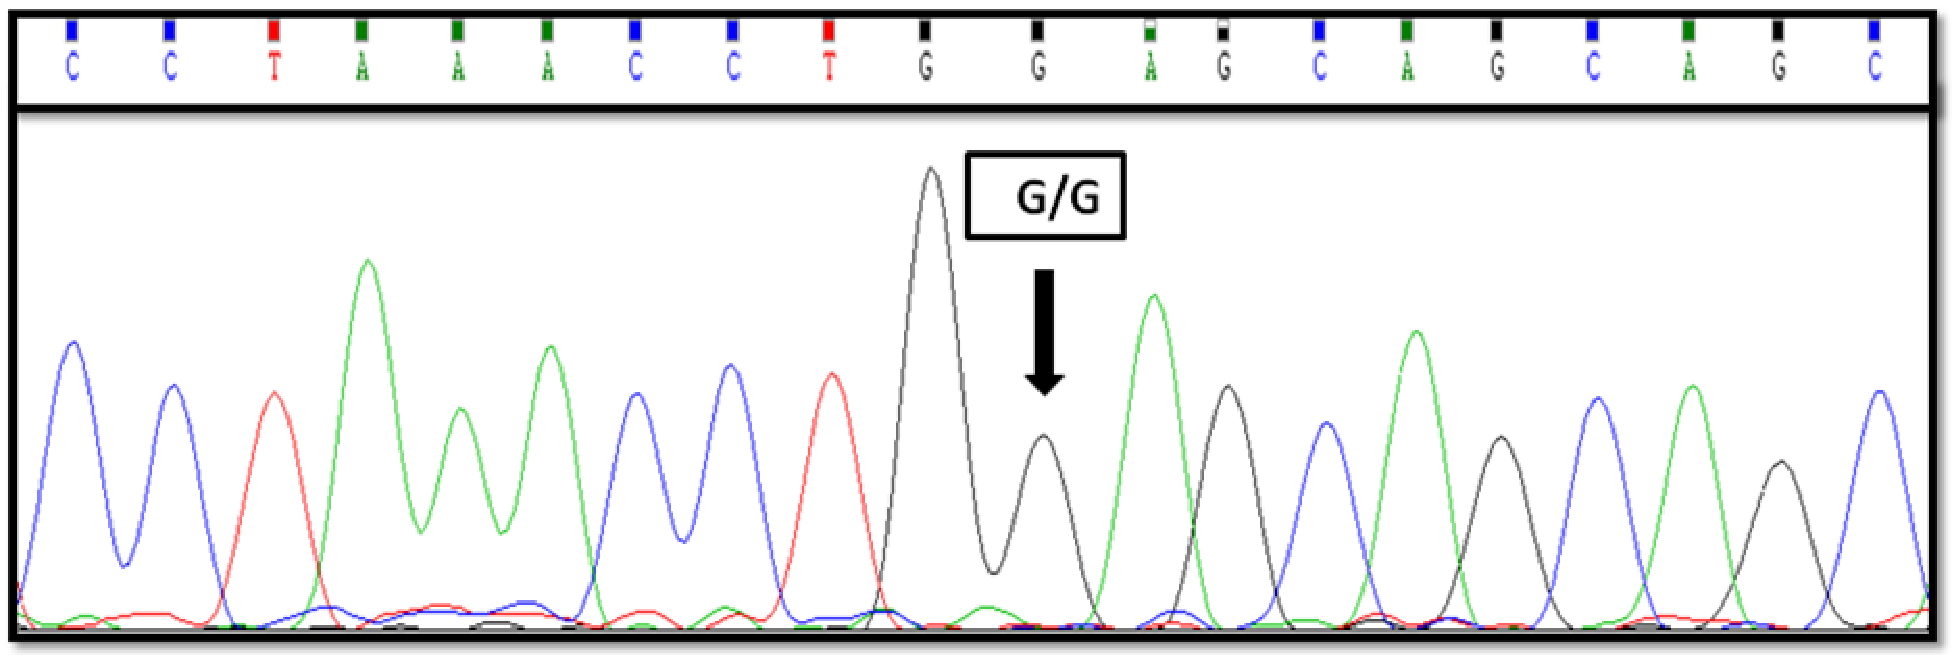
\includegraphics[width=\linewidth]{Figures/Figure5_7.pdf}
\rule{35em}{0.5pt}
\caption{Sequence chromatogram showing the genotype seen with rs104893904}
\label{fig:5_7}
\end{figure}

\begin{figure}[!htb]
\centering
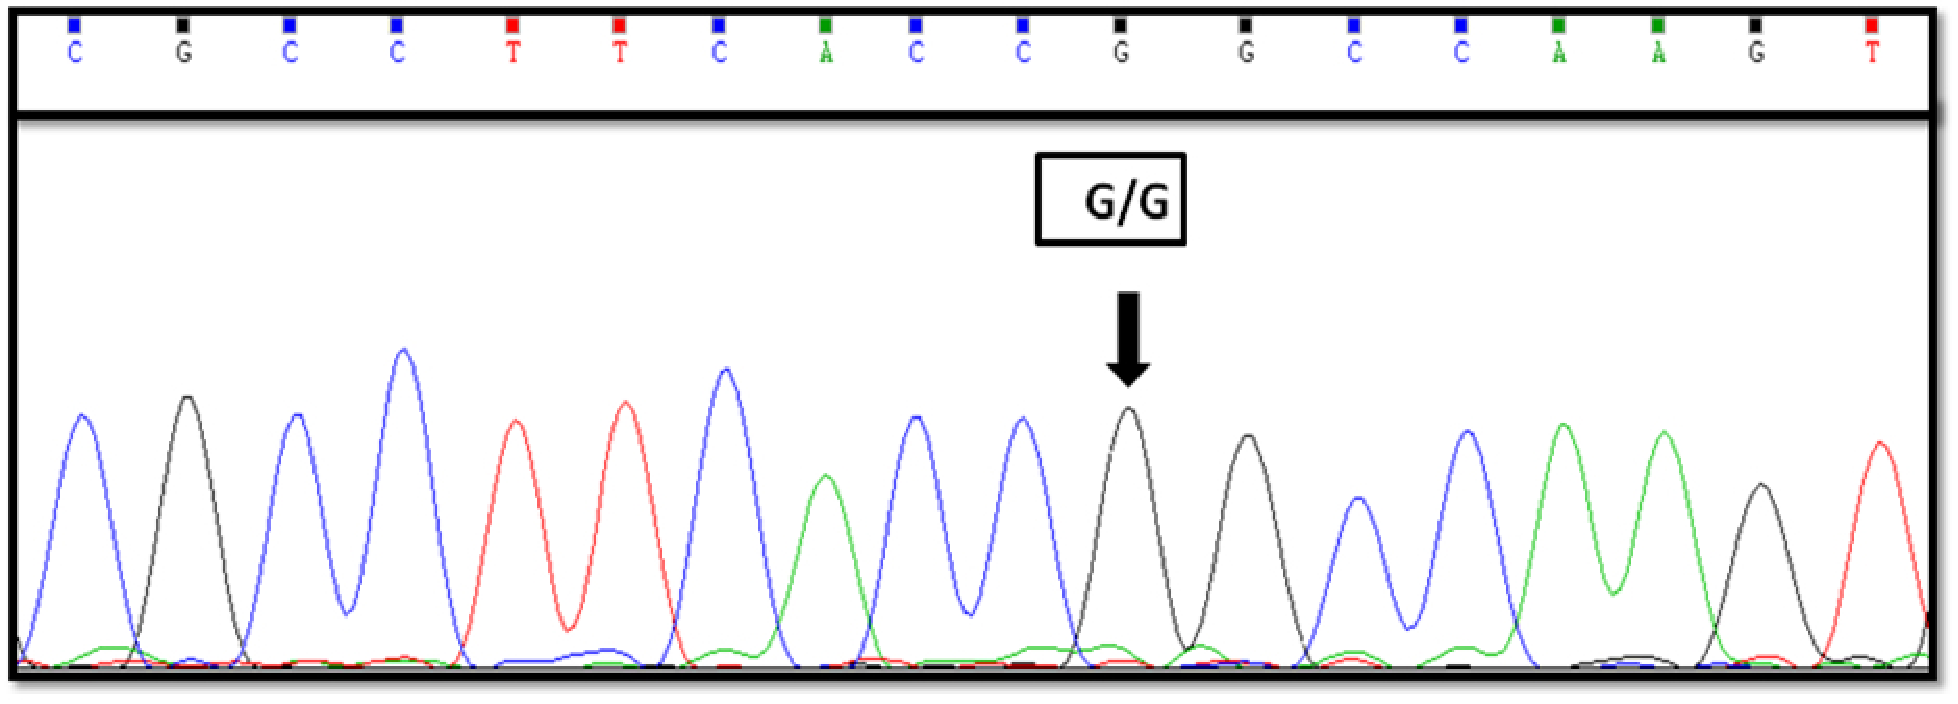
\includegraphics[width=\linewidth]{Figures/Figure5_8.pdf}
\rule{35em}{0.5pt}
\caption{Sequence chromatogram showing the genotype seen with rs72554029}
\label{fig:5_8}
\end{figure}


\begin{figure}[!htb]
\centering
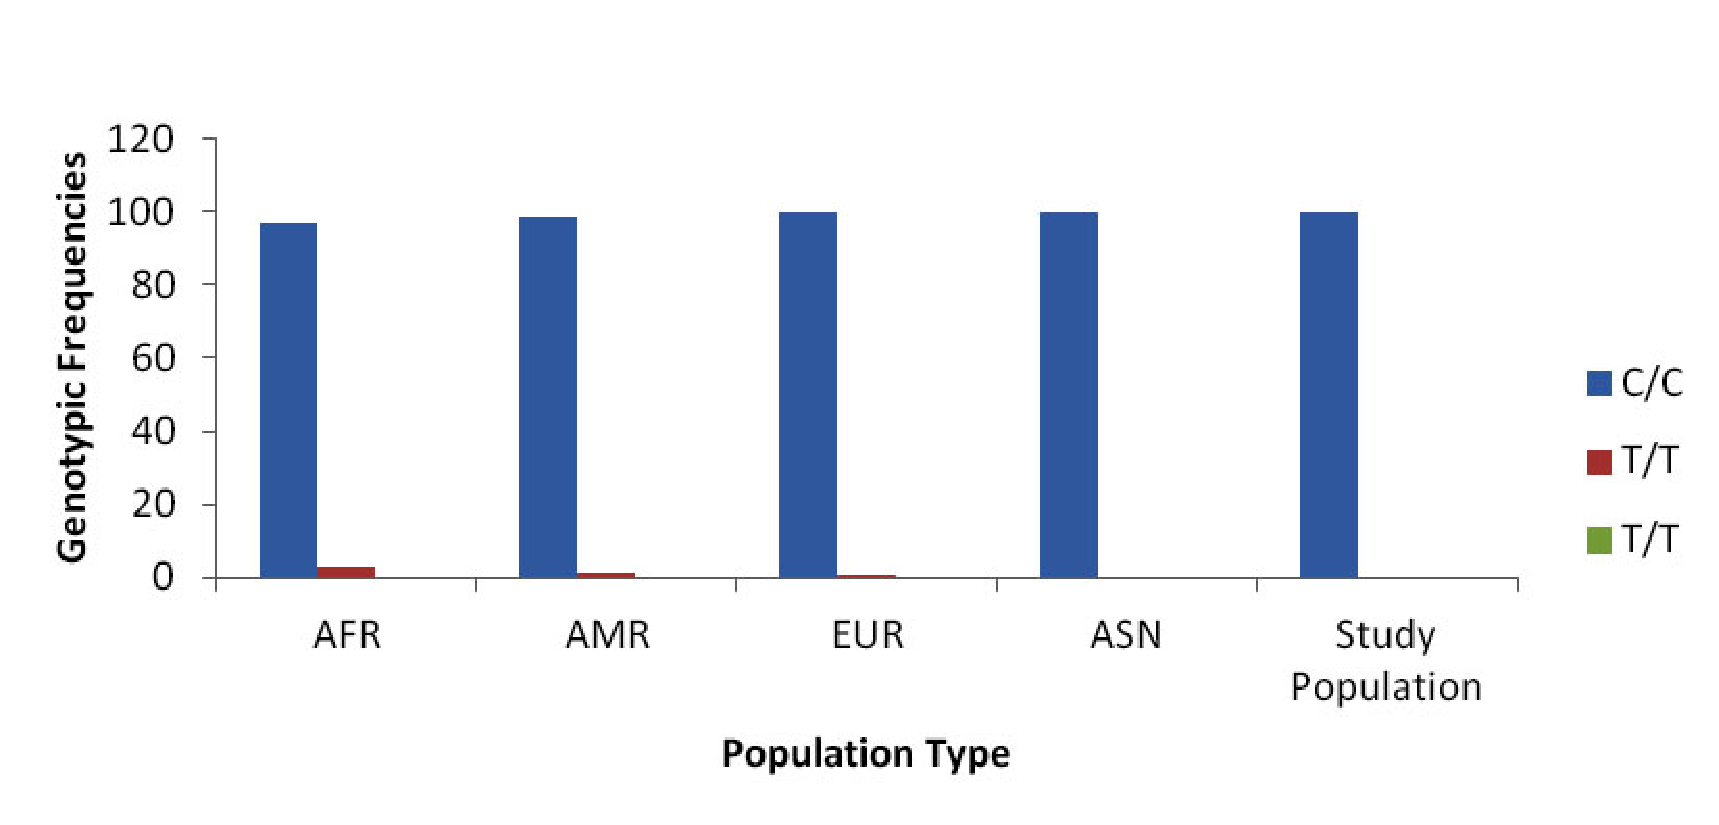
\includegraphics[width=\linewidth]{Figures/Figure5_10.pdf}
\rule{35em}{0.5pt}
\caption{Comparison of rs28936670 distribution in different populations.*\\ {\textsuperscript{*}\footnotesize{AFR:African population; AMR: American; ASN: Asian and EUR: European populations}}}
\label{fig:5_10}
\end{figure}

\begin{figure}[!htb]
\centering
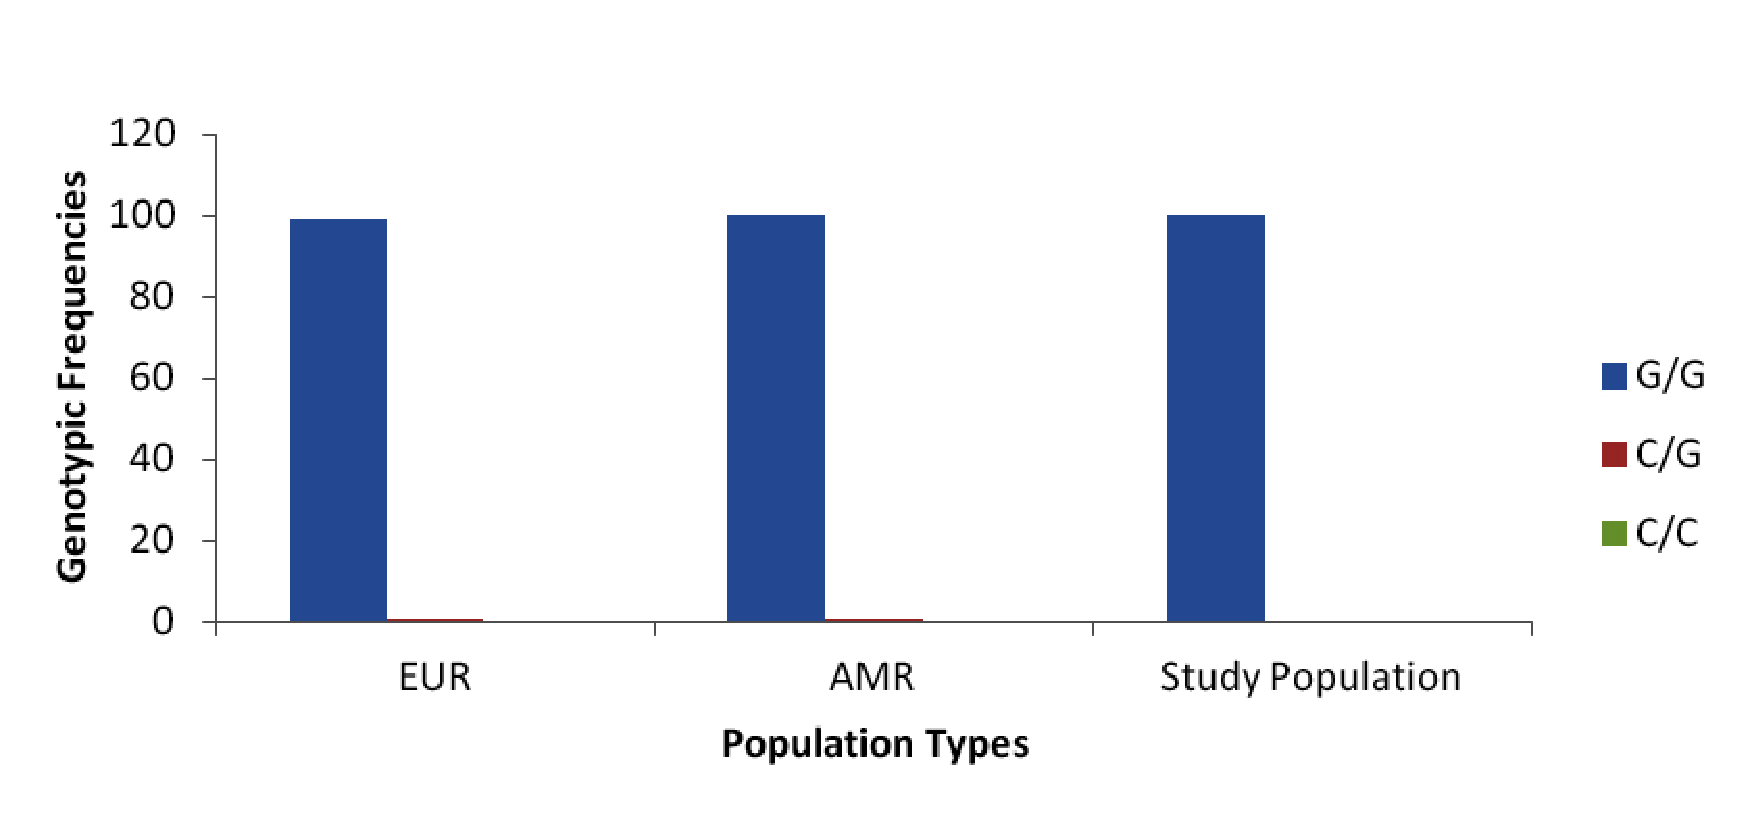
\includegraphics[width=\linewidth]{Figures/Figure5_11.pdf}
\rule{35em}{0.5pt}
\caption{Comparison of rs104893904 distribution in different populations.*\\{\textsuperscript{*}\footnotesize{AFR:African population; AMR: American; ASN: Asian and EUR: European populations}}}
\label{fig:5_11}
\end{figure}

\begin{figure}[!htb]
\centering
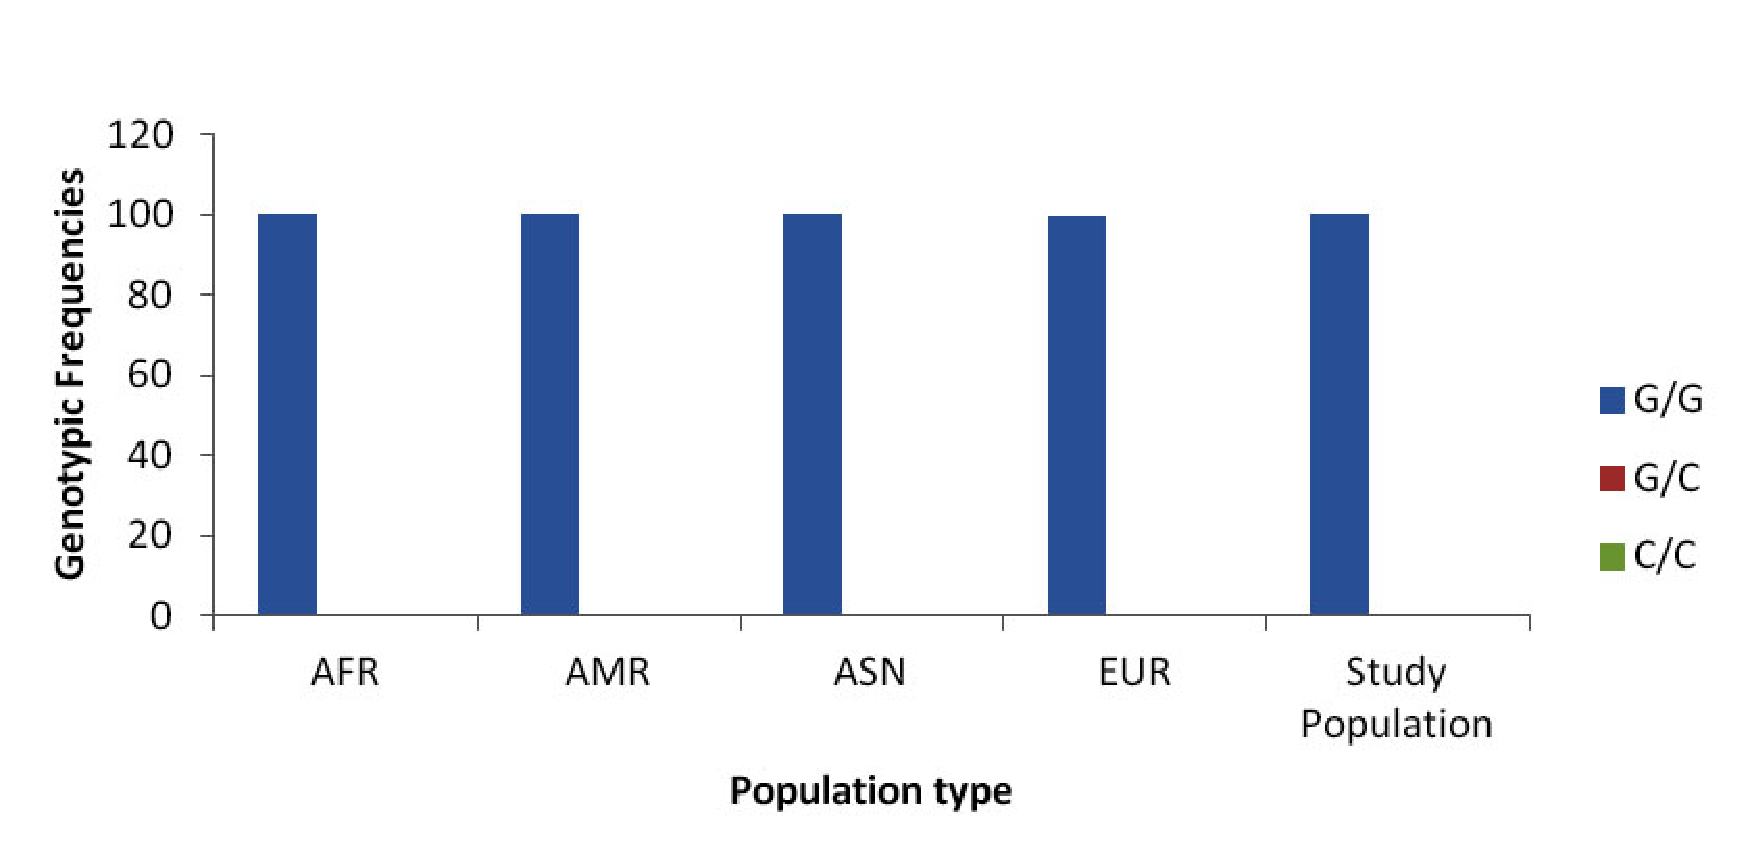
\includegraphics[width=\linewidth]{Figures/Figure5_12.pdf}
\rule{35em}{0.5pt}
\caption{Comparison of rs72554029 distribution in different populations.*\\{\textsuperscript{*}\footnotesize{AFR:African population; AMR: American; ASN: Asian and EUR: European populations}}}
\label{fig:5_12}
\end{figure}

\begin{table}[!tb]
\centering
\caption{Details of rs28936670, rs104893904 and rs72554029}
\label{tab:5_9}
\begin{tabular}{ P{0.9in} P{0.75in} P{0.75in} P{2.3in} }
\toprule
	\textbf{SNP} & \textbf{Nucleotide change} & \textbf{AA change} & \textbf{Genotype observed} \\ \toprule
	rs28936670 & c.25C>T & Arg>Cys & Homozygous wild genotype (CC) \\ \midrule
	rs104893904 & c.21C>G & Gln>Glu & Homozygous mutant type (GG) \\ \midrule
	rs72554029 & c.79G>A & Pro>Pro & Homozygous wild genotype (GG) \\ \bottomrule
\end{tabular}
\end{table}

\subsection{\textit{NKX2.5} expression analysis in tissue versus blood}

The level of the expression of \textit{NKX2.5} obtained from the blood and tissues of cases is given in \cref{tab:5_10}. The expression of the \textit{NKX2.5} gene was significantly higher (p=0.0074) in the tissue samples than in the blood samples. 

\begin{table}[!tb]
\centering
\caption{ΔCt values calculated for the CHD blood and tissue samples}
\label{tab:5_10}
\begin{tabular}{ l  l  l }
\toprule
		 & \textbf{Blood Samples (N=55)} & \textbf{Tissue Samples(N=55)} \\ \toprule
	Average ΔCt & 9.908 & 8.505 \\ \bottomrule
\end{tabular}
\end{table}

However, the averages expression levels of \textit{NKX2.5} in tissues and blood showed inter-individual variation. \cref{fig:5_13} summarizes the individual \textit{NKX2.5} expression levels seen in the study population. For 9 individuals, expression of \textit{NKX2.5} was equal in blood and tissue; for 18 individuals, the expression of \textit{NKX2.5} was lower in tissue than in blood; and for 19 individuals, \textit{NKX2.5} expression was higher in tissue than in blood.

\begin{figure}[!htb]
\centering
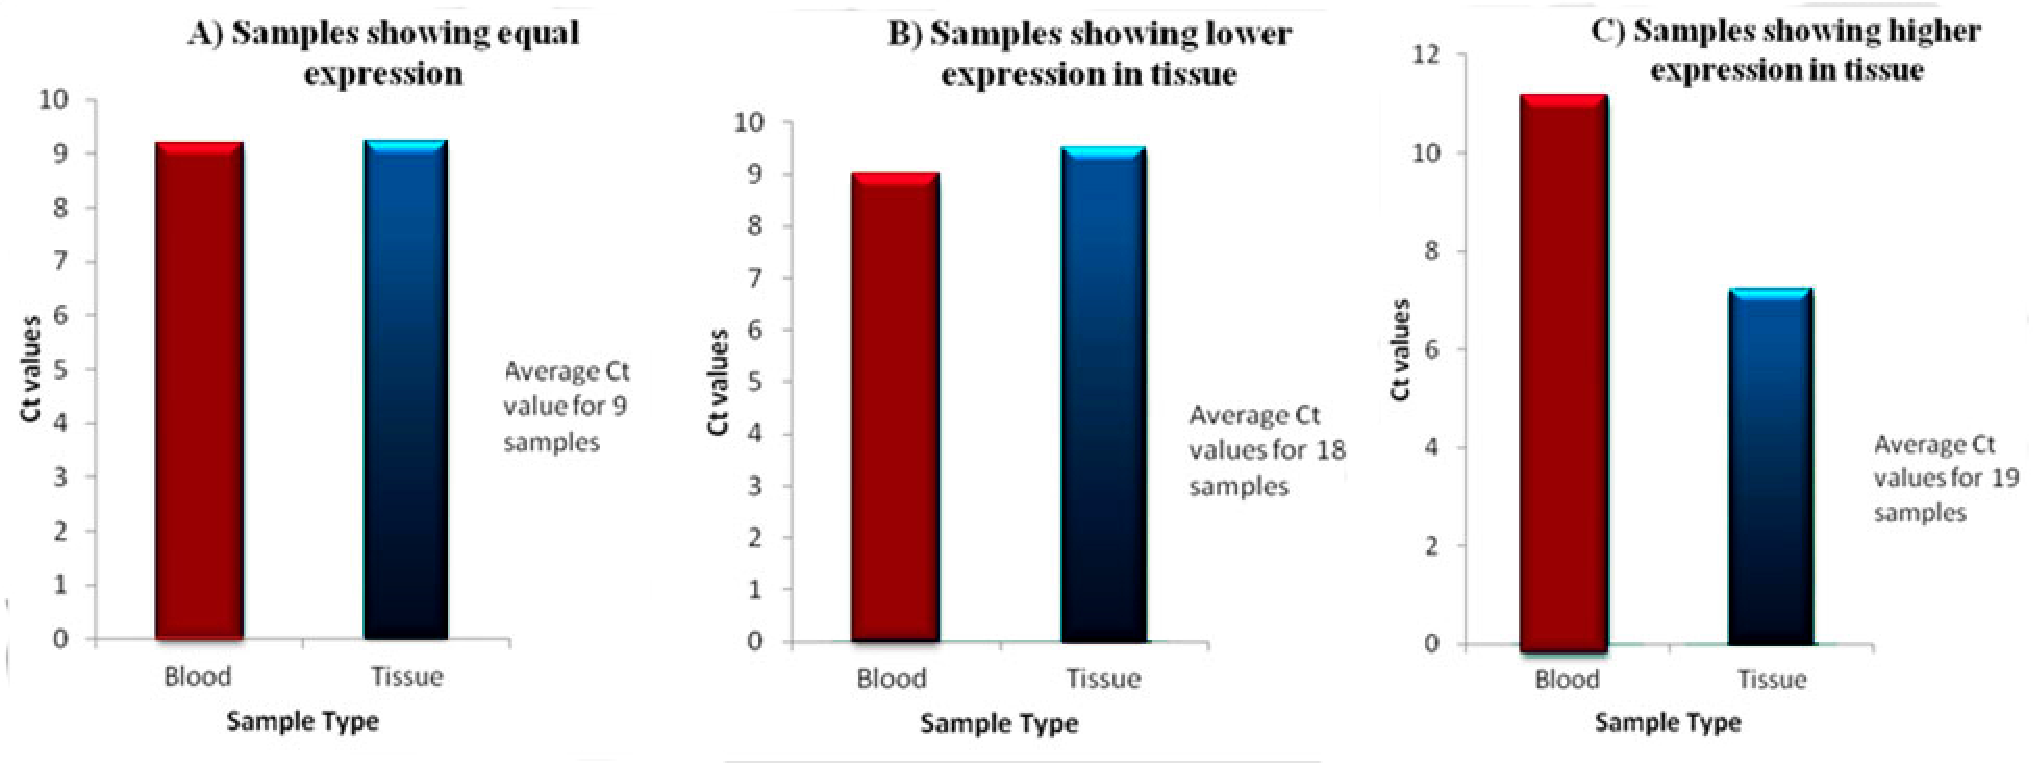
\includegraphics[width=\linewidth]{Figures/Figure5_13.pdf}
\rule{35em}{0.5pt}
\caption{Comparison of C$_t$ values of blood and tissue between individuals}
\label{fig:5_13}
\end{figure}

\section{Discussion}

\textit{NKX2.5} is an important transcription factor for cardiac morphogenesis and development. It regulates several other genes that are involved in heart formation and functioning. So far more than 40 different mutations have been identified in cases with different types of CHDs, both germline and sporadic. Other variations in the gene include SNPs distributed at various positions along the length of the gene. 

In this study, 11 novel \textit{NKX2.5} mutations were detected in the lymphocytic DNA of 21 cases, including 10 with TOF, 4 with TA, 3 with TGA and two each with IAA and DORV. Eight of the sequence alterations were non-synonymous and predicted to change highly conserved amino acids. Given that these variants change highly conserved amino acids and were not identified in normal controls, they were considered to be significant mutations and not random changes. It is known that control populations are not in Hardy-Weinberg genetic equilibrium, because they are exposed to all environmental conditions. Therefore, it can be inferred that genetic changes in cases with CTHD which is not recorded in controls are significant even if they are seen in a single individual of a study population. \cref{tab:5_11} summarizes the mutations reported till date, and the unique mutations observed in this study add to the list of cardiac malformations. The most notable finding of this study was the frequency of mutations in patients with TOF which is higher than the 4\% previously reported by Goldmuntz et al \cite{goldmuntz2001nkx2}.

Seven of the mutation-positive patients had extracardiac anomalies or syndromic features which ranged from mild dysmorphism to considerable developmental delay. However, because of the small number of genotype positive patients a satisfactory correlation could not be established. In addition, all the individuals with a mutation had no known family history of CTHD implying the isolated nature of the CTHD in this study population.


\begin{spacing}{1}
\begin{longtable}{P{0.75in} P{0.9in} P{0.85in} P{1.2in} p{1.3in}}
\caption{Previously reported \textit{NKX2.5} mutations in CHD}\\

%\begin{tabular}
           \toprule
          \textbf{Reference}
        & \multicolumn{2}{c}{\textbf{Mutation}}
        
        & \textbf{Site}
        & \textbf{CHD phenotype}
        \\*
        
        & \textbf{Nucleotide Change}
        & \textbf{Amino acid Change}
        &
        &
        \\* \toprule
	\endhead
 \label{tab:5_11}
%\begin{tabular}
	 \multirow{7}{*}{\cite{benson1999mutations}} & C554T & Gln149ter & Homeodomain & ASD, VSD \\ 
	& C674G    & Arg189Gly & Homeodomain & ASD \\ 
	 & C886A     & Tyr259ter & 3’ – coding region & ASD, VSD \\ 
	 & A681G  & Tyr191Cys & Homeodomain & ASD,VSD \\ 
	 & C673A & Asn188Lys & Homeodomain & ASD \\ 
	 & Int1DSG+1T & - & Splice site & AV block \\ 
	 & C182T & Arg25Cys & 5’ - coding region & TOF \\ \midrule
	 
	\multirow{4}{*}{\cite{goldmuntz2001nkx2}} & G61C & Glu21Gln & \multirow{4}{*}{NK2 domain}  & Stenosis \\ 
	 & C73T & Arg25Cys &  & Stenosis, Atresia \\ 
	 & C646T & Arg216Cys &  & Stenosis \\ 
	 & C656T & Ala219Val &  & Atresia \\ \midrule
	
	 \multirow{12}{*}{\cite{reamon2004somatic,reamon2004novel}}& T196C & Leu7Pro & Exon 1 & AVD \\ 
	 & A232G & Asn19Ser &  & VSD \\ 
	 & C249T & Arg25Cys &  & VSD \\ 
	 & T309C & Ser45Pro &  & VSD \\ 
	 & T327C & Phe51Leu &  & VSD \\ 
	 & T382C & Leu69Pro &  & VSD \\ 
	 & C406T & Pro77Leu &  & VSD \\ 
	 & T516A & Cys114Ser &  & ASD, AVSD \\ 
	 & T516C & Cys114Arg &  & ASD,VSD, AVSD \\ 
	 & A529G & Lys118Arg & Exon 2 & ASD, VSD \\ 
	 & A547G & Lys124Arg &  & VSD \\ 
	 & A553T & Glu126Val &  & ASD, VSD,AVSD \\ 
	 \multirow{27}{*}{\cite{reamon2004somatic,reamon2004novel}} & C573T & Pro133Ser &  & VSD \\ 
	 & G579A & Ala135Thr &  & ASD, AVSD \\ 
	 & T607C & Leu144Pro &  & ASD, AVSD \\ 
	 & C709T & Thr178Met &  & VSD \\ 
	 & A723G & Lys183Glu &  & ASD, AVSD \\ 
	 & C735T & Gln187Ter &  & VSD \\ 
	 & A751C & Lys192Thr &  & VSD \\ 
	 & A751G & Lys192Arg &  & VSD \\ 
	 & A757G & Lys194Arg &  & VSD \\ 
	 & T790A & Val205Glu &  & VSD \\ 
	 & C832T & Ala219Val &  & VSD \\ 
	 & G852A & Asp226Asn &  & VSD \\ 
	 & T918C & Tyr248His &  & VSD \\ 
	 & T1011C & Ser279Pro &  & VSD \\ 
	 & C1012T & Ser279Phe &  & VSD \\ 
	 & C1018T & Ala281Val &  & ASD, VSD,AVSD \\ 
	 & C1033T & Ala286Val &  & ASD, VSD,AVSD \\ 
	 & A1056C & Asn294His &  & ASD \\ 
	 & A1072G & Asp299Gly &  & ASD, VSD,AVSD \\ 
	 & A1089G & Ser305Gly &  & VSD \\ 
	 & G1134A & Gly320Ser &  & ASD, VSD,AVSD \\ 
	 & G1141A & Arg322Gln &  & VSD \\ 
	 & T1149C & STOP-Gln &  & ASD, VSD,AVSD \\ 
	 & A239G & Glu21Glu &  & ASD, AVSD \\ 
	 & C560T & Asp128 Asp &  & ASD, AVSD \\ 
	 & G614T & 146Ser &  & ASD, VSD,AVSD \\ 
	 & T629C & 151Tyr &  & VSD \\ 
	 \multirow{10}{*}{\cite{reamon2004somatic,reamon2004novel}}& A677G & 167Glu &  & VSD \\ 
	 & C680T & 168Arg &  & VSD \\ 
	 & A704G & 176Lys &  &  \\ 
	 & T779C & 201Thr & Exon 1, 5’ UTR &  \\ 
	 & C902G & 242Gly &  &  \\ 
	 & T995C & 273Ala & Exon 2, 3’UTR &  \\ 
	 & C1034T & 286Ala &  &  \\ 
	 & T1079C & 301Asn &  &  \\ 
	 & A1118G & 314Gly &  &  \\ 
	 & A1142G & 322Arg &  &  \\ 
	  \midrule
	\multirow{12}{*}{\cite{mcelhinney2003nkx2}} & A44T & Lys15Ile & TN domain & ASD \\ 
	 & G61C & Glu21Gln & 5’coding region & TOF \\ 
	 & A65C & Gln22Pro & NK domain & TOF \\ 
	 & C73T & Arg25Cys & 3’coding region & TOF,TA, IAA, Hypoplastic \\ 
	 & C188T & Ala63Val &  & TGA \\ 
	 & C380A & Ala127Glu &  & Secundum ASD \\ 
	 & C646T & Arg216Cys &  & TOF \\ 
	 & C656T & Ala219Val &  & TOF \\ 
	 & InsTCCCT701 & D235AFSter &  & Secundum SD; \\ 
	 & C823A & Pro275Thr &  &  \\ 
	 & delAAC871 & del291Asn &  &  \\ 
	 & G967A & Ala323Thr &  &  \\ \midrule
	\multirow{2}{*}{\cite{schott1998congenital}} & C618T & Gln170ter & Homeodomain & Secundum ASD, \\ 
	 & C642T & Thr178Met & Homeodomain & AV Block \\ 
	 \cite{schott1998congenital}& C701T & Gln198ter & 3’ Coding region & Secundum ASD, AV Block \\ 
	  \midrule
	\multirow{3}{*}{\cite{watanabe2002two}} & 215-221- &         - & 5’coding & ASD, VSD, \\ 
	 & delAGCTG &  & region & Heterotaxia, MV \\ 
	 & GG &  &  & Abnormality \\ \midrule
	\cite{elliott2003cardiac} & C642T & Thr178Met & Homeodomain & ASD in association with HLHS \\ \midrule
	 
	\multirow{3}{*}{\cite{hirayama2005phenotypes}} & c.262delG & Ala88Xfs & Exon 1 & AV block, ASD \\ 
	 & C568T & Arg190Cys & Exon 2 - & ASD \\ 
	 & C533T & Thr178Met & Homeodomain & AV block, ASD \\ \midrule
	\multirow{2}{*}{\cite{sarkozy2005spectrum}} & 498-499insC & - & Homeodomain & ASD, AV block \\ 
	 & 605-606delTG & - &  & AV block \\ 
	 & G554T & Trp185Leu &  & ASD,VSD \\ \midrule
	\cite{draus2009investigation} & A65G & Glu22Arg & Exon1 & ASD \\ \midrule
	 
	\multirow{3}{*}{\cite{reamon2013transcriptional}} & C356A & A119E & Homeodomain & AVSD \\ 
	 & G355T & A119S &  & HLHS \\ 
	 & G543A & Q181 &  & AVSD \\ \bottomrule
\end{longtable}
\end{spacing}

Six sequence variants were observed in the hiomeodomain covered by exon 2 .In the majority of previously reported cases such mutations were predicted to alter the coding sense in the homeodomain resulting in a truncated protein \cite{akazawa2005cardiac,benson1999mutations,goldmuntz2001nkx2}. Kasahara and colleagues \cite{kasahara2004biochemical,kasahara2000loss,kasahara2001progressive} have evaluated nuclear localization, DNA binding and transcriptional activation, and dimerization of mutant human \textit{NKX2.5} in vitro and homeodomain mutations demonstrated severely reduced DNA binding and minimal to absent transcriptional activation.

In addition, Schinke et al. \cite{schinke2001lack} examined the effects of cardiac-specific deletion of the \textit{Nk2} domain of \textit{Nkx2.5} in mice. Null mutants died in utero at E14.5 and exhibited a variety of structural cardiovascular anomalies, including VSD, DORV, and AVSD defect, as well as downregulation of the ventricular markers \textit{IRX4} and \textit{MLC-2v}, specifically in the RV. Heterozygous \textit{Nk2} mutant mice, which survived to term, also developed various structural cardiovascular defects. Binding of the \textit{Nk2} mutant protein to DNA was not impaired, and mutant mice did not demonstrate AV conduction abnormalities. These findings suggest that the \textit{NK2} domain also plays an important role in cardiovascular development independent of the homeodomain. The finding of 7 distinct mutations in the 5’ and 3’ coding regions of \textit{NKX2.5} in 5 of 96 patients (5\%) with CTHD, along with the aforementioned experimental findings, suggests that \textit{NKX2.5} mutations outside of the homeodomain, either alone or in conjunction with modifying factors, may also cause CTHD.  Interestingly, case \# 66 presenting with TOF, had multiple mutations which included 1 synonymous mutation and 3 non-synonymous mutations. The non-synonymous mutation was predicted to result in a truncated protein that has the potential for a dominant-negative or deleterious gain of function effects.

Additional studies are required to identify the mechanism by which the novel mutations identified in the present study affect transcription factor function and thereby affect cardiac development. Notably, the remarkable genetic heterogeneity of CTHD was proven by an inability to detect mutations in nearly 80\% of our cases, prompting the consideration of somatic \textit{NKX2-5} mutations being a likely mechanism of CTHD in some cases. The somatic mutations observed in this study included a heterozygous single nucleotide change and two deletion mutations constituting a mutational frequency of 10.9\%. Differences in the frequency of mutations were observed in studies considering cases with a family history of CHD when compared with studies that disregarded familial CHD. While the former reported only one \textit{NKX2.5} mutation in a familial ASD, the latter estimated the frequency as 3\% \cite{mcelhinney2003nkx2,dinesh2010single}.

The somatic c.195C>A sequence variant was found in the tissue DNA of 6 patients. It is predicted that this sequence alteration could be disease causing affecting protein features and splice site changes. Although the mutation was predominately seen in cases with TOF-PA, again the limited number of cases that were mutation positive did not allow for a detailed genotype-phenotype correlation. Some investigators have reported that somatic \textit{NKX2-5} mutations, which have been found in diseased heart tissue, may play a role in non-familial CHD \cite{reamon2004somatic,reamon2004novel,inga2005functional}. Germline mutations in the homeodomain of \textit{NKX2.5} are associated with highly penetrant inherited ASD with AV block \cite{mcelhinney2003nkx2,sarkozy2005spectrum} and TOF \cite{goldmuntz2001nkx2}. The specific variation observed in this study has not been previously reported and considering that it was not recorded in the controls, a larger sample size could clarify the clinical significance of this variation.

\begin{sloppypar} Two deletions which resulted in a frameshift mutation, c.139\_139delA and c.155
\_155delA were identified in the tissue DNA of one patient diagnosed with TOF-PA. Screening of the blood DNA of the patient did not reveal the deletions, implying a somatic nature of the mutations. Deletion mutations in \textit{NKX2.5} have been previously reported by a number of authors with a range of clinical consequences. In 2002 Watanabe et al \cite{watanabe2002two} reported a deletion mutation delAGCTGGG from 215-221 positions in 5’coding region in DORV diagnosed cases. Hirayama-Yamada et al \cite{hirayama2005phenotypes} identified c.262delG resulting in a frameshift mutation in exon 1 of \textit{NKX2.5} in cases diagnosed with ASD. Similarly, McElhinney et al \cite{mcelhinney2003nkx2} observed a deletion mutation, delAAC871, which resulted in a deletion of asparagine at the 291 position in ASD patients. However, the presence of two inherited mutations in a patient, observed in this study, is rare and often only seen in cancers. Hypothetically the mutation reported here could probably result in a truncated non-functional protein mutation. However, we cannot determine with certainty if this mutation is the disease causing mutation or a disease-associated mutation. What is noteworthy is that all the mutations observed in the cardiac tissue were not seen in the blood samples of the same CTHD patients, reiterating the conclusion of studies by Buettner and Borlak \cite{reamon2004somatic,reamon2004novel,inga2005functional} that have reported that \textit{NKX2.5} gene mutations are mosaic in nature. \end{sloppypar}

Association of compromised \textit{NKX2.5} with increased predisposition to CHD has also been reported in animal models. The homeobox-containing transcription factor encoded by the tinman gene, a counterpart of NKX2-5, was expressed in the dorsal vessel (an equivalent to the heart of vertebrates) of the fruit fly Drosophila melanogaster and the deletion of the transcription factor led to lethal failure of vessel formation \cite{benson1999mutations}. In \textit{Xenopus}, expression of a similar DNA-nonbinding mutant of \textit{Nkx2.5} was demonstrated to cause dominant negative effect on embryos, showing small heart or no heart formation \cite{grow1998tinman}. In mice, \textit{Nkx2.5} was highly expressed in the early heart progenitor cells in both primary and secondary heart fields during embryogenesis and continued to be expressed at a high level in the heart through adulthood. In particular, a transiently elevated expression of \textit{Nkx2.5} was observed in specialized myocardial conduction cells during the development of cardiac conduction system \cite{akazawa2005cardiac}. In transgenic mice expressing a DNA binding-impaired mutant of mouse \textit{Nkx2.5} (I183P), under the β-myosin heavy chain promoter, the accumulation of mutant protein in the embryo, neonate, and adult myocardium resulted in progressive and profound cardiac conduction defects and heart failure \cite{kasahara2001progressive}. Targeted disruption of \textit{NKX2.5} in mice caused embryonic lethality around E.10.5, with retarded cardiac development \cite{lyons1995myogenic,tanaka1999cardiac}. Mice heterozygous for \textit{Nkx2.5} null alleles were predisposed to atrial septal defect and abnormal atrioventricular conduction \cite{biben2000cardiac}. In addition, perinatal loss of \textit{Nkx2.5} brought about rapid conduction and contraction defects by regulating expression of several ion channel genes \cite{briggs2008perinatal}. Taken together, these experimental findings in animals suggest that \textit{NKX2.5} mutations underlie a variety of congenital cardiac abnormalities in humans, including atrial septal defect with or without progressive conduction anomaly, ventricular septal defect, and tetralogy of Fallot

In addition to sequence alteration, a synonymous SNP A63G (rs2277923) was identified in the exon-1 region of \textit{NKX2.5} in 30 cases and 7 controls. The A allele frequency was found to 0.59 and the G allele frequency was found to be 0.41 in the CTHD study population. This was in accordance with studies done previously to analyze \textit{NKX2.5} variations in individuals with CTHD \cite{reamon2004somatic}. The odds ratio (95\% CI) for the heterozygous and homozygous variants were 5.83 (2.1126 – 16.1202) and 48.8 (2.7403 – 869.20), respectively. The p value (0.0081 and 0.0007) obtained proved significant, suggesting that the presence of this SNP increases the risk of occurrence of CTHDs. The distribution of genotype frequencies of rs2277923 in the study population was compared with that seen in populations of other ethnicities. The G allele frequency was found to be higher than the A allele in the African, Asian (Chinese and Japanese), while the A allele was predominant in the American, European and the study population.

For the second SNP (rs28936670), only one genotype (CC) was observed in the study population. It has however been reported that only the C allele is almost always present in individuals belonging to other ethnicities also. The other two SNPs, rs104893904 and rs72554029 showed a similar pattern of allele frequency distribution. Analysis of the C61G variant (rs104893904) in the study population showed that only one genotype (GG) was present. No studies have been done for this SNP in the Asian population. Data that exists for the American and European population show that the G allele is predominantly present while the C allele is close to being completely absent. For the rs72554029 variant, only one genotype (GG) was seen in the study population. The G allele frequency was found to be 1 which conforms to the data reported other populations such as African, American, Asian and European populations.

Mutations in the transactivation (TN) and \textit{NK-2} domains have been reported previously in individuals with CTHDs \cite{mcelhinney2003nkx2}. Since these domains are involved in regulating \textit{NKX2.5} gene expression, it follows that there would be changes in the level of \textit{NKX2.5} \cite{inga2005functional}. The expression of the \textit{NKX2.5} gene was analysed in the blood and tissue samples of the CHD study population using RT-PCR. The net Ct values revealed a slight increase in \textit{NKX2.5} expression in the tissue samples in comparison with the blood samples taken from the same individuals. Using a student t-test it was determined that the difference in expression was significant between the blood and tissue samples. Upon comparing the difference in expression in blood and tissue samples separately for each individual, it was found that in 18 CTHD individuals, the gene expression in the blood was higher than in the tissue. Several studies have correlated functional haploinsufficiency or reduced NKX2.5 levels with several CHD phenotypes \cite{sarkozy2005spectrum,briggs2008perinatal}. In 19 CTHD individuals, \textit{NKX2.5} levels were lower in the blood than in the tissue. In a study carried out by Pang et al \cite{pang2012genetic}, it was found that enhanced \textit{NKX2.5} promoter activity was associated with CHD development. Hence, this varied gene expression could be attributed to tissue-specific mutations, probably in the promoter regions or regulatory domains, namely, the TN and NK-2 domain. Determining the exact location of these mutations could help predict their degree of involvement in causing congenital heart disease.

In conclusion, taken together the data suggests that an association between \textit{NKX2.5} and CTHD is present in a small population of cases. Further analysis of \textit{NKX2.5} -mediated regulation of cardiovascular development, as well as functional studies of the mutations that have been identified, is necessary to determine the mechanisms by which \textit{NKX2.5} mutations lead to congenital cardiovascular anomalies. However, screening strategies considering the identification of germline or somatic molecular defects are still largely unwarranted and/or should consider other genes acting in conjunction with \textit{NKX2.5}.


\clearpage
\printbibliography[heading=subbibintoc]
\end{refsection}